% =====================================================================
% 论文 A —— 中文 LaTeX 排版版（IEEE 双栏，Times 10pt，与英文版排布一致）
% 事实源：main.tex（英文排版版，2026-10-01）；术语对齐 docs/paper/论文A-中文初稿.md
% 全部数字为 G3 基准实验锁定值。编译：xelatex（需 texlive-lang-chinese + texlive-xetex）
% =====================================================================
\documentclass[10pt,conference]{IEEEtran}

\usepackage[T1]{fontenc}
\usepackage{textcomp}
\usepackage[UTF8]{ctex}
\usepackage{cite}
\usepackage{times}
\usepackage{mathptmx}
% xelatex 下 times/mathptmx 仅定义 OT1 编码，Latin 需显式指定 TU 编码的 Times 克隆
\usepackage{fontspec}
\setmainfont{TeX Gyre Termes}
\setsansfont{TeX Gyre Heros}
\setmonofont{TeX Gyre Cursor}
\usepackage{amsmath,amssymb}
\usepackage{booktabs}
\usepackage{graphicx}
\usepackage[hidelinks]{hyperref}
\usepackage{url}

\renewcommand{\abstractname}{摘要}
\renewcommand{\tablename}{表}
\renewcommand{\figurename}{图}
\renewcommand{\refname}{参考文献}
\def\IEEEkeywordsname{关键词}

\begin{document}

\title{揭示 OKS-mAP 的评估盲区：面向遮挡、关节角度与时序稳定性的二维人体姿态估计统一评估协议}

\author{
\IEEEauthorblockN{樊一凡}
\IEEEauthorblockA{太原扬帆学校国际部\\中国·太原}
}

\maketitle

\begin{abstract}
二维人体姿态估计的主流评估协议——基于对象关键点相似度（OKS）的 mAP——对三个对下游应用至关重要的性质不敏感：聚合分数不区分可见与遮挡关键点；不度量关节角度误差；对无追踪逐帧推理输出的时序稳定性保持沉默。本文提出一个统一的补充评估协议，包含三个模块：（M1）按真实可见性标注（$v$）分层的 OKS-mAP，并以 $\Delta_{\mathrm{occ}}=\mathrm{mAP}(v{=}1)-\mathrm{mAP}(\mathrm{full})$ 量化聚合指标对遮挡特定差异的掩盖程度；（M2）以真实标注（GT）关键点推导的关节角为参照的角度误差（RMSE/MAE/P95）与膝内扣检出一致性（Cohen's $\kappa$）；（M3）无追踪逐帧推理设定下的帧间位移、中值滤波残差抖动与跳变率，以及 OneEuro 平滑前后的对比。我们在四个公开数据集（COCO val2017、CrowdPose、OCHuman、PoseTrack18）上对两个代表性模型（官方 YOLO11s-pose 与一个遮挡域数据微调模型）执行了协议，全部指标由开源 harness 单次推理统一产出。所有模型-数据集组合的 $\Delta_{\mathrm{occ}}$ 均为负（$-0.24$ 至 $-0.41$）：聚合 mAP 在每一个受测组合中都高估了遮挡场景的表现。角度误差在所有受测组合的遮挡层均被放大；在遮挡域数据集上，角度指标揭示了两模型之间的显著差异，而聚合 mAP 无法定位这一差异。两模型的原始时序抖动未发现差异；像素域 OneEuro 平滑以零精度代价（$|\Delta\mathrm{AP}|\le 0.0002$）将跳变率降低 9--10\%。相关性分析表明分层 mAP 与全量 mAP 高度一致（符号一致性 $\tau_s=1.0$，12/12 对）——其价值在于量级诊断而非重排名——而角度指标（尤其膝角）携带部分独立信息（$\rho=0.72$，$p=0.109$，$n=6$，探索性）。协议与 harness 已开源，定位为 OKS-mAP 的补充而非替代。
\end{abstract}

\begin{IEEEkeywords}
人体姿态估计；评估协议；遮挡；关节角度；时序稳定性；OKS mAP
\end{IEEEkeywords}

\section{引言}

二维人体姿态估计是计算机视觉的基础任务，其输出支撑动作识别、运动分析与实时健身矫正等下游系统。对这些应用而言，基准分数与实际可用性之间的落差比平均精度本身更值得关注：一个在基准上排名领先的模型，可能在人员遮挡、快速运动或需要精细关节角度判断的场景中明显更差——而这一差异在主流指标中不可见。

事实标准评估协议是 COCO keypoints 协议定义的 OKS-mAP~\cite{1}。它以对象关键点相似度（OKS）匹配并计分，在整个测试集上聚合为一个标量。这一设计存在三个盲区。第一，OKS 聚合忽略关键点可见性：可见（$v{=}2$）与遮挡（$v{=}1$）关键点被等权平均进同一分数（缺失关键点 $v{=}0$ 被排除在 OKS 平均之外），遮挡特定的精度差异被平均稀释。第二，协议不度量关节角度：OKS 惩罚的是关键点像素级位置误差，而下游应用（如运动矫正）关心的是由这些关键点推导出的关节角是否准确——两者并非线性对应。第三，协议对时序行为失明：多数系统对视频逐帧独立推理，帧间输出的抖动直接决定下游消费端的观感，而静态图像协议对此完全沉默。已有工作对上述问题各有单点回应——OCHuman 按遮挡级别组织评测~\cite{2}；PoseTrack 与 SmoothNet 分别以跟踪指标（MOTA/MOTP）和时序平滑度指标（逐关节加速度幅值 Accel）延伸了静态协议~\cite{3,15}；生物力学领域验证过 markerless 姿态估计的关节角度~\cite{4,5,6}——但缺少一个统一、可复现、跨数据集的补充协议，也没有任何基准数字说明这三个盲区在真实模型上的量级。

本文提出一个三模块统一补充评估协议（第~3 节），并开源其执行层 eval harness：单次推理同时产出官方指标与协议指标，配三门禁自检。我们在四个公开数据集上以两个代表性模型执行了协议（第~4--5 节），回答四个研究问题：

\begin{itemize}
\item \textbf{RQ1（遮挡）}：全量 OKS-mAP 在多大程度上掩盖遮挡特定的精度差异？按可见性分层后模型排名是否改变？
\item \textbf{RQ2（角度）}：关节角 RMSE 能否提供 OKS-mAP 之外的区分信息？角度误差是否被遮挡放大？
\item \textbf{RQ3（时序）}：无追踪逐帧推理下，模型的时序稳定性差异有多大？平滑能否以可接受的精度代价换取稳定性？
\item \textbf{RQ4（协议精简）}：三模块指标之间以及与全量 mAP 的相关性如何？是否存在冗余？
\end{itemize}

本文贡献有三点：（1）据我们所知，首个将遮挡分层、角度误差与时序抖动统一在一个协议下的补充评估方案，含明确的统计口径（bootstrap 置信区间）与跨数据集一致的分层规则；（2）开源 harness 与全部原始预测，任何新模型可在四个数据集上单次跑出全部协议指标；（3）两个代表性模型的完整基准数字，据我们所知首次量化 OKS-mAP 三盲区的量级（如 COCO 上 $\Delta_{\mathrm{occ}}$ 达 $-0.40$）。

\section{相关工作}

\textbf{姿态估计评估协议。} COCO keypoints 协议以 OKS 为核心，自 2014 年起是该领域的事实标准~\cite{1}。PoseTrack 将评估延伸到视频多人姿态跟踪，建立以 MOTA/MOTP 为核心的跟踪口径~\cite{3}；SmoothNet 更进一步，提出逐关节加速度幅值（Accel，单位像素/帧$^2$）作为视频姿态的时序平滑度指标，并在滤波前后对比中沿用该口径~\cite{15}。本文 M3 与 Accel 互补：Accel 度量帧间二阶差分的大小，而本文的帧间位移与中值滤波残差分别度量位置波动与高频噪声，并额外报告平滑的精度（AP）代价。数据侧，CrowdPose 与 OCHuman 提供真实标注的可见性/遮挡标签（CrowdPose 的 $v{=}1$；OCHuman 的三级遮挡）~\cite{2,7}。这些工作的共同边界是：各自在单一数据集、单一维度上做单点改进，没有形成跨数据集统一口径的补充协议。

\textbf{遮挡鲁棒性评估。} 已有工作尝试量化遮挡对姿态估计的影响：Ghafoor 与 Mahmood 通过合成移除关节构造三组实验，量化遮挡对 3D 姿态误差的影响~\cite{8}；后续工作在合成遮挡下的鲁棒性评测~\cite{9}与可见性感知的视频遮挡基准~\cite{10}上延续这一思路。与本文的差异：这些工作使用合成遮挡或非真实标注的分层，且集中于单数据集、单指标；本文直接利用三个数据集的真实 $v$ 标注跨数据集分层，并对照全量 mAP 报告 $\Delta_{\mathrm{occ}}$。

\textbf{关节角度验证。} 生物力学与运动科学领域有一条 markerless 姿态估计效度研究线：Turner 等在 89 段阻力训练视频上以 BlazePose 关键点重建关节角轨迹，按逐帧 RMSE 对照参考动作评估动作技术质量~\cite{4}；Panconi 等验证 DeepLabCut 在步态分析中的关节角~\cite{5}；Pemasiri 等构建面向生物力学解释的步态分析框架~\cite{6}。这些研究回答的问题是「估测角度是否等于临床/标记点金标准」（效度），需要专门的标记点或专家标注。本文不重复效度验证，而是把 GT 推导角度用作模型间比较的协议指标。两条线互补而非竞争（第~6 节详述边界）。膝内扣阈值取文献量级参照：侧向下台阶测试的额状面投影角（FPPA）16.0--17.4$^{\circ}$~\cite{11}。

\textbf{时序一致性与平滑。} 无追踪逐帧推理的时序不一致问题由 Deep Video Prior 等从通用层面讨论~\cite{12}；工程实践中广泛采用 OneEuro 因果滤波平滑关键点轨迹~\cite{13}。本文把「无追踪原始输出的稳定性」本身变成协议指标，并对比两种滤波域（归一化坐标域与像素域）对抖动指标与 AP 的联合影响——这一对比揭示了滤波域选择如何决定平滑的收益与代价。

\section{协议设计}

\subsection{总览}

协议由三个模块加一个统计层组成，全部建立在 COCO 17 关键点定义与 OKS 口径的公共基础之上。表~\ref{tab:overview} 给出总览。

\begin{table}[t]
\centering
\caption{协议总览。}
\label{tab:overview}
\renewcommand{\arraystretch}{1.15}
\resizebox{\columnwidth}{!}{%
\begin{tabular}{p{0.95in}p{0.85in}p{1.15in}p{0.45in}}
\toprule
\textbf{模块} & \textbf{指标} & \textbf{数据} & \textbf{回答} \\
\midrule
M1 遮挡分层 & $v$ 分层 mAP$^{50-95}$(P) + $\Delta_{\mathrm{occ}}$ & CrowdPose val / OCHuman test / COCO val & RQ1 \\
M2 角度误差 & 肘/膝关节角 RMSE/MAE/P95 + 膝内扣检出一致性（$\kappa$） & 同 M1（角度由 GT 推导，零额外标注） & RQ2 \\
M3 时序抖动 & 帧间位移 / 抖动 / 跳变率，OneEuro 前后 & PoseTrack18 val（无追踪逐帧推理） & RQ3 \\
统计层 & 10k bootstrap CI + 符号一致性 $\tau_s$ + Spearman $\rho$ & 三模块结果 & RQ4、模型比较 \\
\bottomrule
\end{tabular}}
\end{table}

\subsection{M1：遮挡分层 mAP}

\textbf{分层口径。} 每个 GT 关键点按其可见性标签 $v$ 归层：$v{=}2$ 可见、$v{=}1$ 遮挡、$v{=}0$ 缺失。层内独立计算 OKS AP。$v{=}0$ 层只报告、不参与排名（该层关键点无法被估计，分数接近零；保留该层作为协议完整性的证据）。每个数据集在转换到 COCO17 后保留真实 $v$ 标注：CrowdPose 官方 14 点映射为 COCO 索引 5--16（head\_top 与 neck 两点丢弃——属映射裁剪而非可见性标签破坏，12 个映射点的 $v{=}1$ 标签完整保留）；OCHuman 官方 test 标注本身即 COCO17 格式，直通保留；COCO val 本身含 $v{=}1$ 标注（占关键点 7.75\%）。

\textbf{计算口径。} 沿用 pycocotools 2.0.11 的 keypoints 协议（官方发布数背后的口径）：OKS 阈值 0.50:0.95 共 10 档取均值；num\_keypoints$=$0 的 GT 标为 ignore；maxDets$=$20。分层只改变统计、不改变匹配逻辑：人员匹配（TP/FP 判定）仍按全关键点 OKS 进行，层 AP 只累计该层 GT 关键点的 OKS 贡献。三门禁保证实现正确（与官方库对拍差 $\le0.0001$；合成自检；分层开关不改变全量 mAP）。

\textbf{解释性证据。} 层 AP 的召回分母为全部 GT 人员，因此没有该层关键点的人员永远无法为该层贡献 TP。故每层同时报告「该层 GT 关键点占比」（gt\_frac）与「拥有该层关键点的 GT 人员占比」（gt\_person\_frac）。特别地，CrowdPose 的 v2 层受 14$\rightarrow$17 映射裁剪影响（gt\_person\_frac 仅 0.591），其 v2 层 AP 被系统性低估——CrowdPose 上 v2 与 v1 的跨层比较应使用 $\Delta_{\mathrm{occ}}$（该指标不受此伪影影响）。

\textbf{主指标。} $\Delta_{\mathrm{occ}}=\mathrm{mAP}(v{=}1\ \mathrm{层})-\mathrm{mAP}(\mathrm{全量})$；为负表示全量指标高估遮挡场景表现。两项均在相同的图像域、相同的全量 GT 人员集上计算（$v{=}1$ 层的召回分母即全量 GT 人员集，见解释性证据），因此 $\Delta_{\mathrm{occ}}$ 隔离的是遮挡层的贡献缺口，而非分母变化。逐层 mAP 与 gt\_frac 一并报告。

\subsection{M2：角度误差}

\textbf{关节角定义。} 以 COCO17 索引定义四个关节（表~\ref{tab:joints}）；内角 $\theta=\arccos\big((\mathbf{a}\cdot\mathbf{b})/(|\mathbf{a}|\,|\mathbf{b}|)\big)$，其中 $\mathbf{a}$、$\mathbf{b}$ 分别为顶点到近端、远端的向量。$|\mathbf{a}|$ 或 $|\mathbf{b}|<10^{-6}$ 的实例剔除。

\begin{table}[t]
\centering
\caption{关节角定义（COCO17 索引，0-based）。}
\label{tab:joints}
\renewcommand{\arraystretch}{1.15}
\begin{tabular}{lcc}
\toprule
\textbf{关节} & \textbf{顶点} & \textbf{端点（近端, 远端）} \\
\midrule
左肘 & 7 & 5, 9 \\
右肘 & 8 & 6, 10 \\
左膝 & 13 & 11, 15 \\
右膝 & 14 & 12, 16 \\
\bottomrule
\end{tabular}
\end{table}

\textbf{有效性掩码。} GT 角度：三个 GT 点 $v$ 均 $>0$ 才计入；预测角度：同三点 GT $v$ 均 $>0$ 且预测置信度 $>0$ 才计入——保证 GT 与预测在同一域上可比，避免偏向缺失预测。逐实例误差 $e=\theta_{\mathrm{pred}}-\theta_{\mathrm{gt}}$；报告 RMSE、MAE 与 P95，按顶点 GT 可见性分 $v{=}2$/$v{=}1$ 两层报告，与 M1 联动。

\textbf{膝内扣检出一致性。} 膝内扣角 $\phi$ 定义为髋$\rightarrow$膝向量与髋$\rightarrow$踝向量在图像平面的夹角（膝点偏离髋-踝轴线的程度），仅对三点 $v$ 均 $>0$ 的实例计算。$\phi_{\mathrm{pred}}$ 与 $\phi_{\mathrm{GT}}$ 按阈值 $\tau_\varphi$ 二值化（默认 $\tau_\varphi=15^{\circ}$，敏感性分析 $\tau_\varphi\in\{10^{\circ},17^{\circ}\}$），以 GT 为金标准报告检出灵敏度、特异度与 Cohen's $\kappa$。两点澄清：不报告绝对检出率（静态数据集视角混杂，绝对率无意义；一致性才是协议能测的量）；$\phi$ 是任意视角下的 2D 图像平面代理量，而 FPPA 文献值来自标准化正面机位~\cite{11}——本文数据集视角混杂，故 $\tau_\varphi$ 仅取文献量级参照，不具临床诊断含义。

\subsection{M3：时序抖动}

\textbf{数据与匹配。} PoseTrack18 val 视频逐帧独立推理（无追踪、无跨帧信息）；每帧预测与 GT 按全关键点 OKS 做匈牙利匹配（口径同 M1）。帧间隔 $>1$ 即断段；仅保留连续 $\ge10$ 帧有匹配的轨迹段。所有位移按 GT 人框尺度 $s_t=\sqrt{w\cdot h}$ 归一化（与 OKS 尺度口径一致）。

\textbf{三指标}（逐关键点、逐轨迹段计算后取均值）：

\begin{enumerate}
\item 帧间位移 $d_t=\lVert\mathbf{p}_t-\mathbf{p}_{t-1}\rVert_2/s_t$：报告均值与 P95；
\item 抖动 $j_t=\lVert\mathbf{p}_t-\hat{\mathbf{s}}_t\rVert_2/s_t$，$\hat{\mathbf{s}}$ 为因果 5 帧中值滤波后的轨迹：专测高频噪声（核心指标）；
\item 跳变率：$d_t>\tau_j$ 的帧占比，默认 $\tau_j=0.10$（人框尺度的 10\%），敏感性 $\tau_j\in\{0.05,0.20\}$。
\end{enumerate}

\textbf{OneEuro 前后对比。} 离线对 $\mathbf{p}_t$ 施加因果 OneEuro 滤波，参数固定为 Casiez 默认值（min\_cutoff$=1.0$、beta$=0.007$、d\_cutoff$=1.0$）~\cite{13}。平滑后重算三指标与匹配口径 AP，报告精度代价。滤波域双口径：归一化坐标域（q 域，协议原设计）与像素域。实证发现（两模型一致）：q 域滤波在反归一化时把 GT 人框的逐帧尺度噪声（$|s_t/s_{t-1}-1|$，中位数 0.97\%，P95 8.1\%）重新注入像素域，导致抖动指标不降反升、AP 微降；像素域直接滤波零 AP 代价且三指标全面下降。\textbf{本文采用像素域为主口径}，q 域作为敏感性口径如实报告（表~\ref{tab:m3} 双列）。

\subsection{统计口径}

\begin{itemize}
\item 模型比较：M1/M2 图像级、M3 轨迹段级重采样，10,000 次 bootstrap（seed 42）；报告差值 $\Delta$ 的 95\% 百分位 CI，以 CI 是否包含 0 判断显著性。M1 为配对设计（共享图像域 $=$ 两模型 GT 图与预测图的并集）；M2/M3 的有效单元集随匹配结果不同，采用独立重采样，协议中已注明。
\item 比较清单在实验前固定（2 模型 $\times$ 3 数据集 $\times$ 层/关节/指标）；每项均报告 CI，不挑选有利结果。
\item RQ4（协议精简）：在（数据集 $\times$ 层）单元上，计算协议指标差与全量 mAP 差的符号一致性 $\tau_s$，并计算两组差值向量之间的 Spearman $\rho$。$\tau_s$ 统计全部两两单元比较中的同号对，排除全量 mAP 差相同的单元对（并列，符号一致性无定义）：$n=6$（3 数据集 $\times$ 2 层）时，15 个两两比较减去 3 个同数据集层对 $=$ 12 个报告对；关节级（$n=24$：3 数据集 $\times$ 4 关节 $\times$ 2 层）时，276 个两两比较减去 84 个同数据集同关节层对（$3\times28$）$=$ 192 个报告对。两项分析均为探索性，样本量已在正文注明。
\end{itemize}

\subsection{Harness 与可复现性}

执行层为开源 eval harness：\texttt{model.val(save\_json=True)} 单次推理同时产出官方指标与预测 JSON；M1/M2/M3 引擎纯离线（NumPy）计算，不占 GPU。三门禁保证口径实现正确（见 3.2 节）。可复现契约（环境、权重、数据、逐条命令、口径说明）见仓库 REPRODUCIBILITY.md。协议 JSON 契约（schema\_version$=$1）可供下游作图与二次分析。harness 与本文源码开源：\url{https://github.com/fanyifan090409-dev/pose-eval-harness} 与 \url{https://github.com/fanyifan090409-dev/elthan-pose-research}；训练分支（基于 ultralytics）见 \url{https://github.com/fanyifan090409-dev/elthan-pose}。

\section{实验设置}

\textbf{数据集。} 四个公开数据集：COCO val2017（通用域对照；$v$ 分布 55.4\%/7.8\%/36.8\% 对应 $v{=}2/1/0$）、CrowdPose val（拥挤/遮挡域；$v{=}1$ 为真实遮挡标记；分布 22.5\%/30.8\%/其余）、OCHuman test（重度遮挡域；分布 69.2\%/14.3\%/其余）、PoseTrack18 val（视频时序；170 视频 / 8,923 标注帧；GT $v\in\{0,1\}$，其中 $v{=}0$ 即 (0,0) 占位）。所有数据集统一为 COCO17 关键点格式。PoseTrack 经 MPII 官方学术许可获取，仅用于学术评估。

\textbf{模型。} 两个基准模型：（1）官方 YOLO11s-pose 预训练权重~\cite{14}；（2）round5-3——在 COCO、MPII、CrowdPose、OCHuman 等公开数据上微调 YOLO11s-pose 所得，代表遮挡域数据训练。两者同架构、同推理配置，仅训练数据不同，适合检验协议对训练数据差异的敏感性。round5-3 的训练数据仅限训练划分（COCO train2017、MPII train、CrowdPose train、OCHuman train，另加受控比例的 OpenThermalPose train）；本文所用的四个评测划分（COCO val2017、CrowdPose val、OCHuman test、PoseTrack18 val）均未出现在其训练数据中，协议数字无泄漏。

\textbf{推理与口径。} 输入 $640\times640$，逐帧独立推理，save\_json 保存预测。所有 mAP 数字采用 pycocotools 2.0.11 官方发布数口径；该口径的 OKS 双倍 bbox 兜底规则：GT 关键点 $vg>0$ 但关键点面积为 0（$k_1=0$，即 COCO (0,0) 占位）时，以 bbox 推导的尺度计分而非直接丢弃。注意该口径与 ultralytics 内部评估器可相差 20 点以上（根源：num\_keypoints$=$0 的 GT 标 ignore、OKS 双倍 bbox 兜底、maxDets$=$20）；论文每张表均注明口径。PoseTrack 无官方 pycoco 对照，其官方指标仅报告内部评估器口径（round5-3 0.1085 / YOLO11s-pose 0.1213 mAP$^{50-95}$(P)）。门禁 1（与官方库对拍）在全部六个模型-数据集单元上实测 $\le 0.0001$（五个单元精确为 0）。

\section{结果}

\subsection{RQ1：全量 mAP 掩盖遮挡差异}

表~\ref{tab:m1} 给出两模型在三个数据集上的分层 mAP，以及层代表性证据 gt\_frac 与 gt\_person\_frac；图~\ref{fig:m1} 可视化分层结果。三点观察。

\begin{table}[t]
\centering
\caption{M1 分层 mAP$^{50-95}$(P)（pycocotools 2.0.11 口径）。粗体 $=$ 显著占优（bootstrap CI 不含 0）。gt\_frac $=$ 该层 GT 关键点占比；gt\_person\_frac $=$ 拥有该层至少一个关键点的 GT 人员占比（两者均为 GT 属性，两模型相同）。$\Delta_{\mathrm{occ}}=$ mAP（$v{=}1$ 层）$-$ mAP（全量），同一全量 GT 人员集上计算（3.2 节）；其 bootstrap CI 见附录~A。--- $=$ 该层不定义。CrowdPose 的 v2 层受 14$\rightarrow$17 映射裁剪影响（gt\_person\_frac 0.591）；跨层比较使用 $\Delta_{\mathrm{occ}}$。}
\label{tab:m1}
\renewcommand{\arraystretch}{1.15}
\resizebox{\columnwidth}{!}{%
\begin{tabular}{lccccccc}
\toprule
\textbf{数据集} & \textbf{层} & \textbf{round5-3} & \textbf{YOLO11s-pose} & \textbf{$\Delta_{\mathrm{occ}}$ (r5-3)} & \textbf{$\Delta_{\mathrm{occ}}$ (YOLO)} & \textbf{gt\_frac} & \textbf{gt\_person\_frac} \\
\midrule
COCO val & full & 0.5712 & \textbf{0.5816} & --- & --- & 1.000 & 1.000 \\
 & $v{=}2$ & 0.5637 & \textbf{0.5728} & --- & --- & 0.554 & 0.988 \\
 & $v{=}1$ & 0.1747 & 0.1719 & $-0.3965$ & $-0.4097$ & 0.078 & 0.564 \\
 & $v{=}0$ & 0 & 0 & --- & --- & 0.368 & 0.947 \\
CrowdPose val & full & \textbf{0.7626} & 0.6938 & --- & --- & 1.000 & 1.000 \\
 & $v{=}2$ & \textbf{0.4183} & 0.3768 & --- & --- & 0.225 & 0.591 \\
 & $v{=}1$ & \textbf{0.5183} & 0.4573 & $-0.2443$ & $-0.2366$ & 0.308 & 0.776 \\
 & $v{=}0$ & 0 & 0 & --- & --- & 0.467 & 1.000 \\
OCHuman test & full & \textbf{0.4775} & 0.3379 & --- & --- & 1.000 & 1.000 \\
 & $v{=}2$ & \textbf{0.4696} & 0.3314 & --- & --- & 0.692 & 1.000 \\
 & $v{=}1$ & \textbf{0.1819} & 0.0765 & $-0.2955$ & $-0.2614$ & 0.143 & 0.736 \\
 & $v{=}0$ & 0 & 0 & --- & --- & 0.164 & 0.902 \\
\bottomrule
\end{tabular}}
\end{table}

第一，\textbf{$\Delta_{\mathrm{occ}}$ 全部为负且量级可观}：COCO 上 $-0.40$ 与 $-0.41$，CrowdPose $-0.24$，OCHuman $-0.26$ 至 $-0.30$。在每一个受测组合中，全量 mAP 都高估了遮挡场景表现 24--41 个点——这一量级足以在仅凭 mAP 做模型选择时掩盖实质差异。

第二，\textbf{分层改变了模型比较的结论强度}。通用域 COCO 上，YOLO11s-pose 在全量与 $v{=}2$ 层显著占优（$\Delta=+0.0104$，95\% CI $[0.0059,0.0155]$），但 $v{=}1$ 层未发现差异（$\Delta=-0.0028$，ns）——聚合分数上的显著优势几乎全部来自可见关键点。遮挡域数据集上，round5-3 三层全部显著占优（CrowdPose 全量 $\Delta=-0.0687$，OCHuman 全量 $\Delta=-0.1396$，95\% CI 均不含 0），遮挡域训练的收益在 $v{=}1$ 层同样显著（OCHuman v1 $\Delta=-0.1055$）。

第三，\textbf{$v{=}0$ 层恒为 0}（两模型、三数据集），验证协议预期：缺失关键点无法被估计；该层保留作完整性证据，不参与排名。

\subsection{RQ2：角度误差与膝内扣检出一致性}

表~\ref{tab:m2} 给出左右侧合并的肘/膝关节角 RMSE（按 $v{=}2$/$v{=}1$ 分层）；图~\ref{fig:m2} 展示逐关节误差分布（$v{=}2$ 层）。三点观察。

\begin{table}[t]
\centering
\caption{M2 关节角 RMSE（$^{\circ}$，左右侧按样本数合并）。粗体 $=$ 显著占优（bootstrap CI 不含 0）；逐项比较的 CI 见附录~A（表~A3）。}
\label{tab:m2}
\renewcommand{\arraystretch}{1.15}
\resizebox{\columnwidth}{!}{%
\begin{tabular}{lccccc}
\toprule
\textbf{数据集} & \textbf{模型} & \textbf{肘 $v{=}2$} & \textbf{肘 $v{=}1$} & \textbf{膝 $v{=}2$} & \textbf{膝 $v{=}1$} \\
\midrule
COCO val & round5-3 & 26.0 & 35.9 & 20.4 & 29.2 \\
 & YOLO11s-pose & 25.4 & 35.6 & 21.0 & 31.2 \\
CrowdPose val & round5-3 & 25.9 & \textbf{31.6} & 20.6 & \textbf{25.9} \\
 & YOLO11s-pose & 26.0 & 35.0 & 21.3 & 30.5 \\
OCHuman test & round5-3 & \textbf{35.6} & \textbf{45.7} & \textbf{24.3} & \textbf{32.0} \\
 & YOLO11s-pose & 39.6 & 57.7 & 28.3 & 39.7 \\
\bottomrule
\end{tabular}}
\end{table}

第一，\textbf{角度误差被遮挡系统性放大}：每个模型-数据集组合中，$v{=}1$ 层 RMSE 均高于 $v{=}2$ 层（肘 $+5.7^{\circ}$ 至 $+18.1^{\circ}$，膝 $+5.3^{\circ}$ 至 $+11.4^{\circ}$），层间差距在重度遮挡域（OCHuman）最大。这与 M1 的 $\Delta_{\mathrm{occ}}$ 观察同向，两者互为佐证。

第二，\textbf{角度指标区分了全量 mAP 无法区分的信息}。通用域 COCO 上未发现两模型角度差异的证据（与 mAP 差 1 点一致）；但遮挡域上 round5-3 在 $v{=}1$ 层每一项受测比较中都更准：CrowdPose 肘 31.6$^{\circ}$ vs.\ 35.0$^{\circ}$、膝 25.9$^{\circ}$ vs.\ 30.5$^{\circ}$（均显著）；OCHuman 肘 45.7$^{\circ}$ vs.\ 57.7$^{\circ}$、膝 32.0$^{\circ}$ vs.\ 39.7$^{\circ}$（全部显著）。注意 OCHuman 的 $v{=}2$ 层角度差异同样显著，说明遮挡域训练的收益不限于被遮挡关键点本身。

第三，\textbf{膝内扣检出一致性}（表~\ref{tab:kappa}）：round5-3 的 $\kappa$ 在三个数据集上均高于 YOLO11s-pose（COCO 0.759 vs.\ 0.745；CrowdPose 0.739 vs.\ 0.669；OCHuman 0.602 vs.\ 0.519），阈值敏感性分析（$\tau_\varphi\in\{10^{\circ},17^{\circ}\}$）下结论稳定。Bootstrap CI（附录~A，表~A4）确立 CrowdPose 与 OCHuman 的差距显著（$\Delta\kappa$ $-0.069$ [$-0.098$, $-0.041$] 与 $-0.084$ [$-0.121$, $-0.046$]），COCO 的差距方向一致但不显著（$\Delta\kappa$ $-0.014$ [$-0.045$, $0.016$]）。两模型在 OCHuman 上的 $\kappa$ 均偏低（$<0.61$），提示重度遮挡下 $\phi$ 的测量噪声上升。

\begin{table}[t]
\centering
\caption{膝内扣检出一致性（二值化 $\phi$ vs.\ GT）。粗体 $=$ 更高值（round5-3）；$\kappa$ 及模型差的 bootstrap CI 见附录~A。}
\label{tab:kappa}
\renewcommand{\arraystretch}{1.15}
\resizebox{\columnwidth}{!}{%
\begin{tabular}{lccccc}
\toprule
\textbf{数据集} & \textbf{模型} & \textbf{$\tau_\varphi{=}10^{\circ}$ $\kappa$} & \textbf{$\tau_\varphi{=}15^{\circ}$ $\kappa$} & \textbf{$\tau_\varphi{=}17^{\circ}$ $\kappa$} & \textbf{$\tau_\varphi{=}15^{\circ}$ 灵敏度/特异度} \\
\midrule
COCO val & round5-3 & 0.724 & \textbf{0.759} & 0.773 & 0.790/0.950 \\
 & YOLO11s-pose & 0.697 & 0.745 & 0.759 & 0.783/0.943 \\
CrowdPose val & round5-3 & 0.711 & \textbf{0.739} & 0.731 & 0.785/0.937 \\
 & YOLO11s-pose & 0.666 & 0.669 & 0.665 & 0.722/0.926 \\
OCHuman test & round5-3 & 0.601 & \textbf{0.602} & 0.603 & 0.646/0.926 \\
 & YOLO11s-pose & 0.529 & 0.519 & 0.502 & 0.592/0.900 \\
\bottomrule
\end{tabular}}
\end{table}

\subsection{RQ3：无追踪推理的时序稳定性与平滑代价}

PoseTrack18 val 上两模型各得到 704 / 728 条轨迹段（161 / 160 个视频，中位段长 31 帧）。表~\ref{tab:m3} 给出 person-scale 归一化后的总体三指标与平滑 AP 代价；图~\ref{fig:m3} 展示一条示例轨迹。

\begin{table}[t]
\centering
\caption{M3 时序指标（总体，17 关键点平均）与平滑 AP 代价。匹配口径 AP 为在抖动指标所用同一批匹配轨迹帧上重算的 AP（原始值：round5-3 0.1316 / YOLO11s-pose 0.1408）；--- $=$ 原始参照，未施加平滑。粗体 AP 代价 $=$ 位于零的 $\pm0.0002$ 内（零精度代价）。逐指标的域间差与模型间差 CI 见附录~A（表~A5）。}
\label{tab:m3}
\renewcommand{\arraystretch}{1.15}
\resizebox{\columnwidth}{!}{%
\begin{tabular}{lcccccc}
\toprule
\textbf{模型} & \textbf{口径} & \textbf{disp\_mean} & \textbf{jitter\_mean} & \textbf{jump\_0.05} & \textbf{jump\_0.10} & \textbf{AP 代价} \\
\midrule
round5-3 & 原始 & 0.0409 & 0.0521 & 0.2062 & 0.0726 & --- \\
 & 像素域平滑 & 0.0380 & 0.0509 & 0.1870 & 0.0634 & \textbf{$+0.0001$} \\
 & q 域平滑 & 0.0432 & 0.0528 & 0.2200 & 0.0807 & $-0.0013$ \\
YOLO11s-pose & 原始 & 0.0430 & 0.0535 & 0.2153 & 0.0777 & --- \\
 & 像素域平滑 & 0.0399 & 0.0523 & 0.1943 & 0.0679 & \textbf{$+0.0002$} \\
 & q 域平滑 & 0.0462 & 0.0546 & 0.2336 & 0.0878 & $-0.0029$ \\
\bottomrule
\end{tabular}}
\end{table}

三点观察。第一，\textbf{两模型的原始时序稳定性未发现差异}：全部七个指标（位移/抖动均值与 P95、三档跳变率阈值）的 bootstrap CI 均包含 0。未发现遮挡域训练数据改变时序稳定性的证据——「未发现遮挡训练影响时序行为的证据」本身即一个有信息量的结果，提示数据侧干预应与时序后处理分开考虑。

第二，\textbf{像素域 OneEuro 平滑以零精度代价换取稳定性}：跳变率（$\tau_j=0.05$）相对下降 9.3\%（round5-3）与 9.7\%（YOLO11s-pose），帧间位移均值下降约 7\%，AP 变化保持在 $\pm0.0002$ 内。第三，\textbf{q 域平滑适得其反}：三指标全面上升（jump\_0.05 升至 0.2200/0.2336），AP 微降——GT 人框的逐帧尺度噪声在反归一化时被重新注入像素域（机制见 3.4 节）。这一对比说明：对无追踪逐帧输出做平滑时，滤波域的选择决定收益；协议因此固定像素域为主口径。

\subsection{RQ4：指标间相关性}

在（数据集 $\times$ 层）单元（$n=6$）上，计算协议指标差（$\Delta=$ YOLO11s-pose $-$ round5-3，RMSE 差经符号翻转使正值恒代表 YOLO11s-pose 更优）与全量 mAP 差的符号一致性 $\tau_s$，仅统计全量 mAP 差互不相同的 12 对（3.5 节）：分层 mAP $\tau_s=1.0$（12/12 对），肘角 RMSE $\tau_s=1.0$（12/12），膝角 RMSE $\tau_s=0.667$（10/12）；扩展到 24 个关节级单元，$\tau_s=0.719$（165/192）。同一差值向量之间的 Spearman $\rho$：全量 $\Delta$ 与分层 $\Delta$ 之间 $\rho=0.956$（$p=0.003$）；全量 $\Delta$ 与肘角之间 $\rho=0.956$（$p=0.003$）；全量 $\Delta$ 与膝角之间 $\rho=0.717$（$p=0.109$）；肘角与膝角之间 $\rho=0.771$（$p=0.072$）。两个相同的 $\rho=0.956$ 并非转录错误：分层 mAP 与肘角误差的差值向量对六个单元的排序完全相同，且它们与全量 mAP 差的排序差异仅发生在同一数据集的两个层之间——该两层共享同一个全量 mAP 差（并列），Spearman 分子在两种情况下均不变。

两点解读（探索性；$n=6$ 已如实标注）。第一，\textbf{分层 mAP 的排名信息与全量 mAP 完全符号一致（$\tau_s=1.0$）}；其协议价值不在重排名，而在量级诊断——$\Delta_{\mathrm{occ}}$ 提供的「被掩盖多少」是标量 mAP 无法给出的。第二，\textbf{角度指标携带部分独立信息}：膝角 RMSE 与全量 AP 的相关性未达显著，且在 COCO 上方向分歧（round5-3 膝角更准而全量 mAP 更低；表~\ref{tab:m2}）——角度协议捕获了 OKS 之外的差异维度。就协议精简而言：分层 mAP 与角度误差均不冗余，各自捕捉不同盲区。时序指标仅有一个数据集的单元，待更多数据检验。

\section{讨论}

\textbf{三盲区的量级据我们所知首次在同一协议下被量化。} 四个数据集、两个模型的一致观察是：全量 mAP 对遮挡场景的高估（$\Delta_{\mathrm{occ}}$ $-0.24$ 至 $-0.41$）、遮挡对角度误差的放大（$v{=}1$ 层肘角 RMSE 最高 $+18.1^{\circ}$）、以及无追踪逐帧输出的高频抖动（跳变率 $\approx0.21$，可被像素域平滑零代价降低约 10\%）。这些数字共同说明：仅由 OKS-mAP 驱动的模型选择，在最需要可靠的场景（遮挡、快速运动）上，可能对两个受测模型的相对强弱做出与分层证据相悖的判断。

\textbf{角度协议与效度研究的边界。} 本文的角度指标以 GT 推导角度为参照，回答「哪个模型的关节角更接近标注真值」——一种模型比较工具。它不验证「估测角度是否等于临床金标准」，后者是 markerless 效度文献~\cite{4,5,6}的任务，需要标记点或专家标注。两者互补：效度研究证明某个模型在特定场景可信，本协议则让任何新模型在标准数据集上获得角度维度的可比较分数。同样，膝内扣检出一致性（$\kappa$ 最高 0.76）只断言「与 GT 标注一致」，不断言临床意义。

\textbf{时序指标的工程含义。} M3 的两个发现直接指导系统设计：其一，数据侧干预（遮挡训练）不改变时序稳定性，时序质量必须单独处理；其二，平滑域选择决定收益——归一化域滤波看似理论正确，实际因 GT 框尺度噪声重注入而失效。协议固定像素域主口径，并建议任何时序平滑方法报告「平滑前后抖动 + AP 代价」的联合表。

\textbf{局限。} （1）基准仅覆盖两个同架构模型，本文不声称覆盖模型空间——协议价值在于口径与工具，更多模型的基准数字留待后续工作；（2）CrowdPose 的 v2 层受 14$\rightarrow$17 映射裁剪影响，该数据集上跨层比较使用 $\Delta_{\mathrm{occ}}$；（3）角度为 2D 图像平面角，受视角影响，不是 3D 关节角或临床角度；（4）M3 仅覆盖一个数据集，时序结论的普适性待扩展；（5）RQ4 相关分析的单元数小（$n=6$），属探索性；（6）COCO 的 $v{=}1$ 层仅占关键点 7.8\%，其 $v{=}1$ 层估计方差较大（CI 更宽）。每张表均注明评估口径：M1/M2 数字遵循 pycocotools 2.0.11，而 PoseTrack 的官方指标数字（第~4 节）因无官方 pycoco 对照而以 ultralytics 内部评估器口径报告。

\section{结论}

本文提出并执行了一个面向遮挡、关节角度与时序稳定性的二维人体姿态估计统一补充评估协议，配套开源 harness 与可复现契约。两个模型、四个公开数据集上的基准结果显示：在每一个受测的模型-数据集组合中，全量 OKS-mAP 都掩盖了遮挡特定的精度差异（$\Delta_{\mathrm{occ}}$ 达 $-0.41$）；角度误差协议捕获了 OKS 之外的部分独立信息；像素域平滑能以零精度代价降低时序抖动。协议定位为 OKS-mAP 的补充而非替代：它不改变主流排名的底层口径，而是为模型选择与系统设计增加三个此前不可见的诊断维度。代码与全部原始预测已开源。

% =====================================================================
% 图（与英文版同一套图文件）
% =====================================================================

\begin{figure*}[t]
\centering
\begin{minipage}[b]{0.32\linewidth}
  \centering
  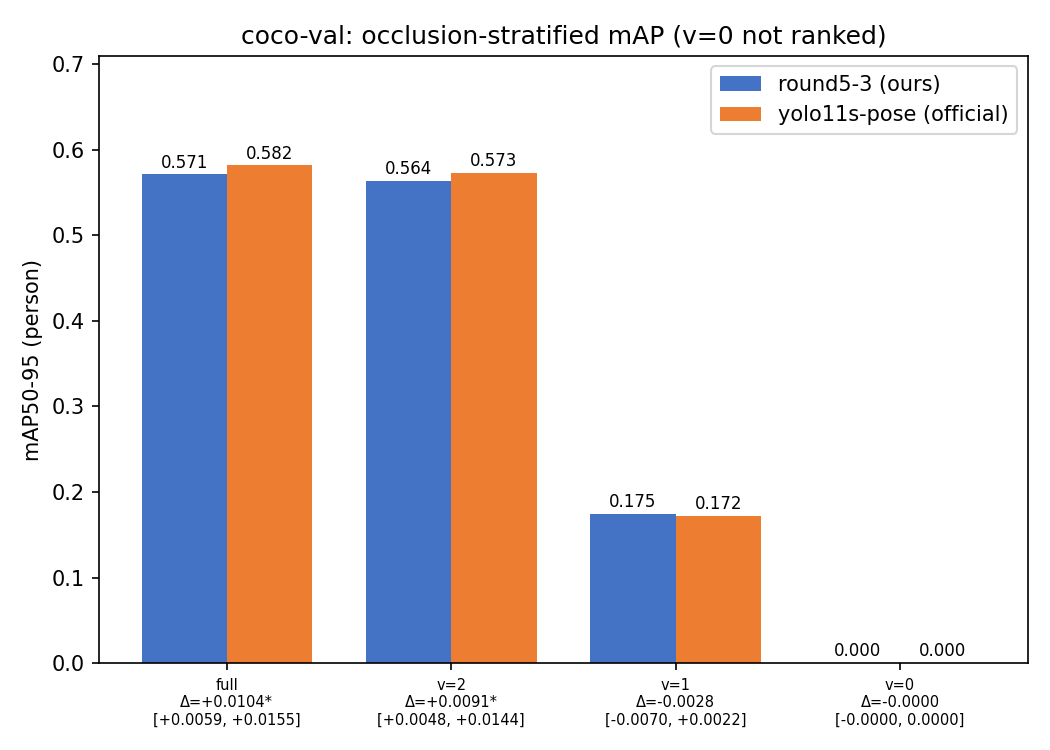
\includegraphics[width=\linewidth]{figures/fig_m1_coco-val.png}
\end{minipage}\hfill
\begin{minipage}[b]{0.32\linewidth}
  \centering
  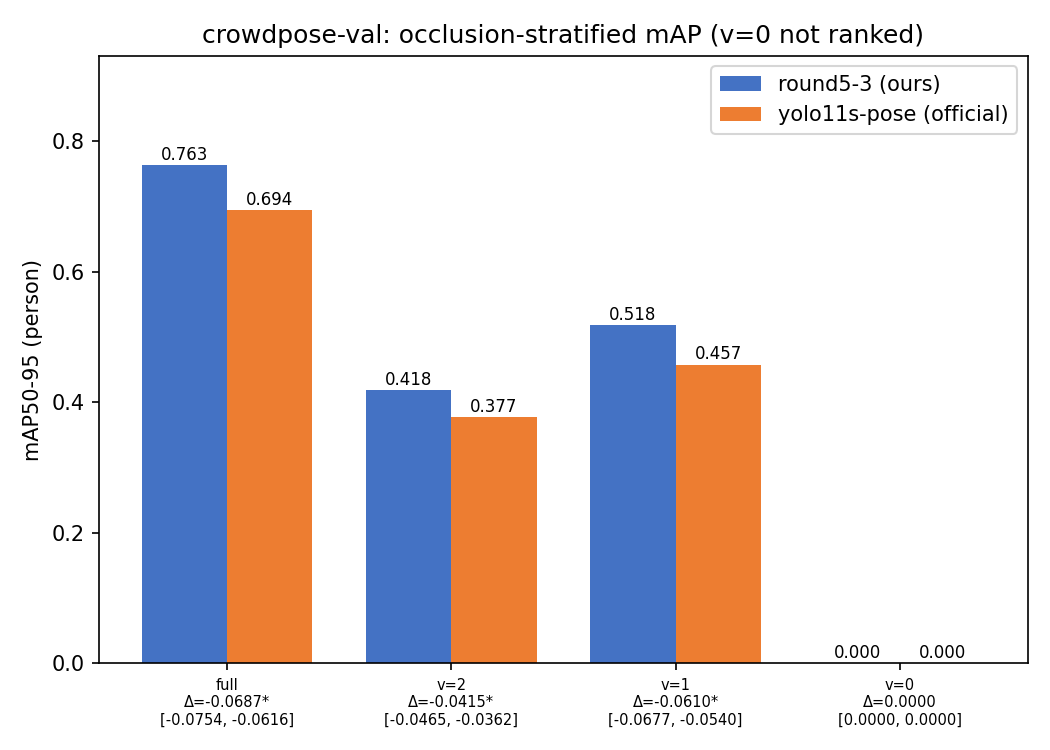
\includegraphics[width=\linewidth]{figures/fig_m1_crowdpose-val.png}
\end{minipage}\hfill
\begin{minipage}[b]{0.32\linewidth}
  \centering
  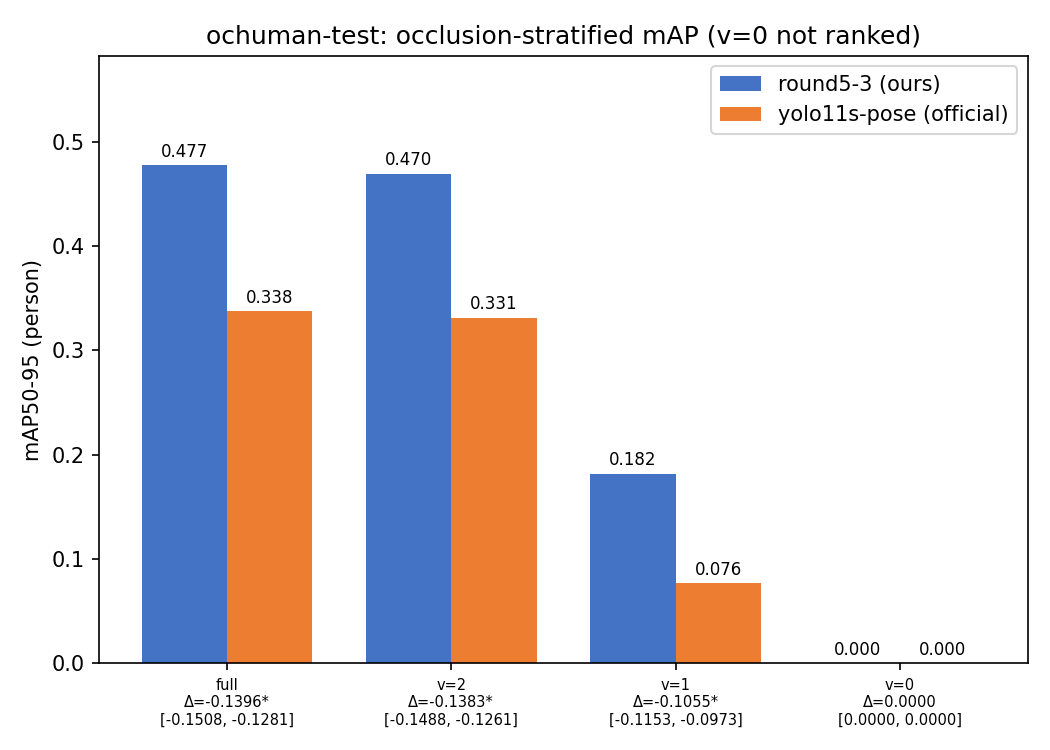
\includegraphics[width=\linewidth]{figures/fig_m1_ochuman-test.png}
\end{minipage}
\caption{M1 遮挡分层 mAP$^{50-95}$(P)（分数据集）：(a) COCO val2017，(b) CrowdPose val，(c) OCHuman test。柱状图展示 round5-3 与 YOLO11s-pose 的全量与逐层 mAP；每组下方标注两模型差值 $\Delta$ 及其 95\% bootstrap CI（$*$ $=$ CI 不含 0）。$v{=}0$ 层为完整性展示，不参与排名。}
\label{fig:m1}
\end{figure*}

\begin{figure*}[t]
\centering
\begin{minipage}[b]{0.32\linewidth}
  \centering
  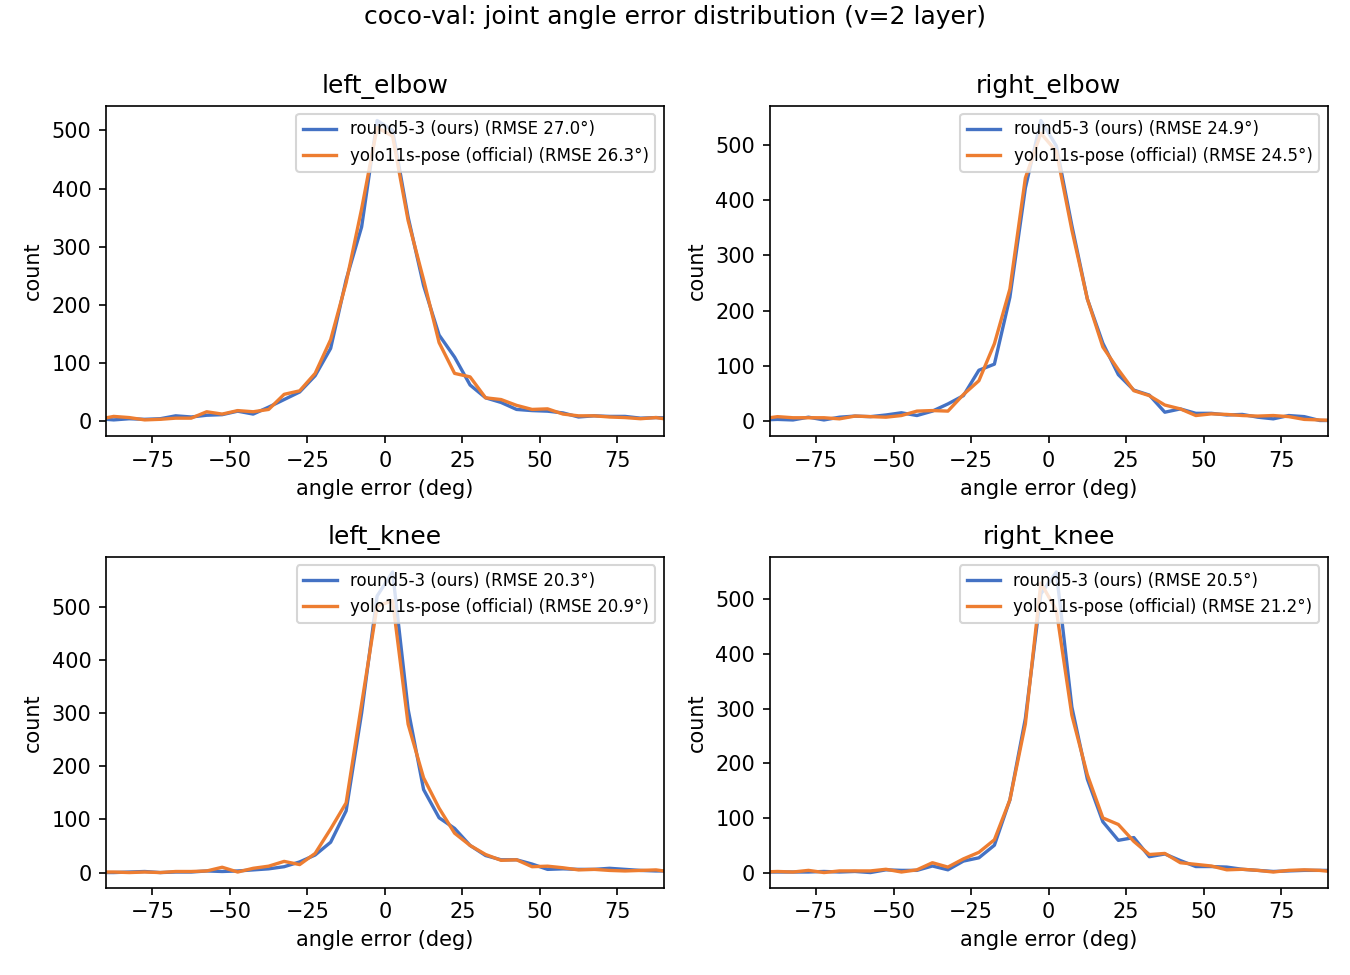
\includegraphics[width=\linewidth]{figures/fig_m2_coco-val.png}
\end{minipage}\hfill
\begin{minipage}[b]{0.32\linewidth}
  \centering
  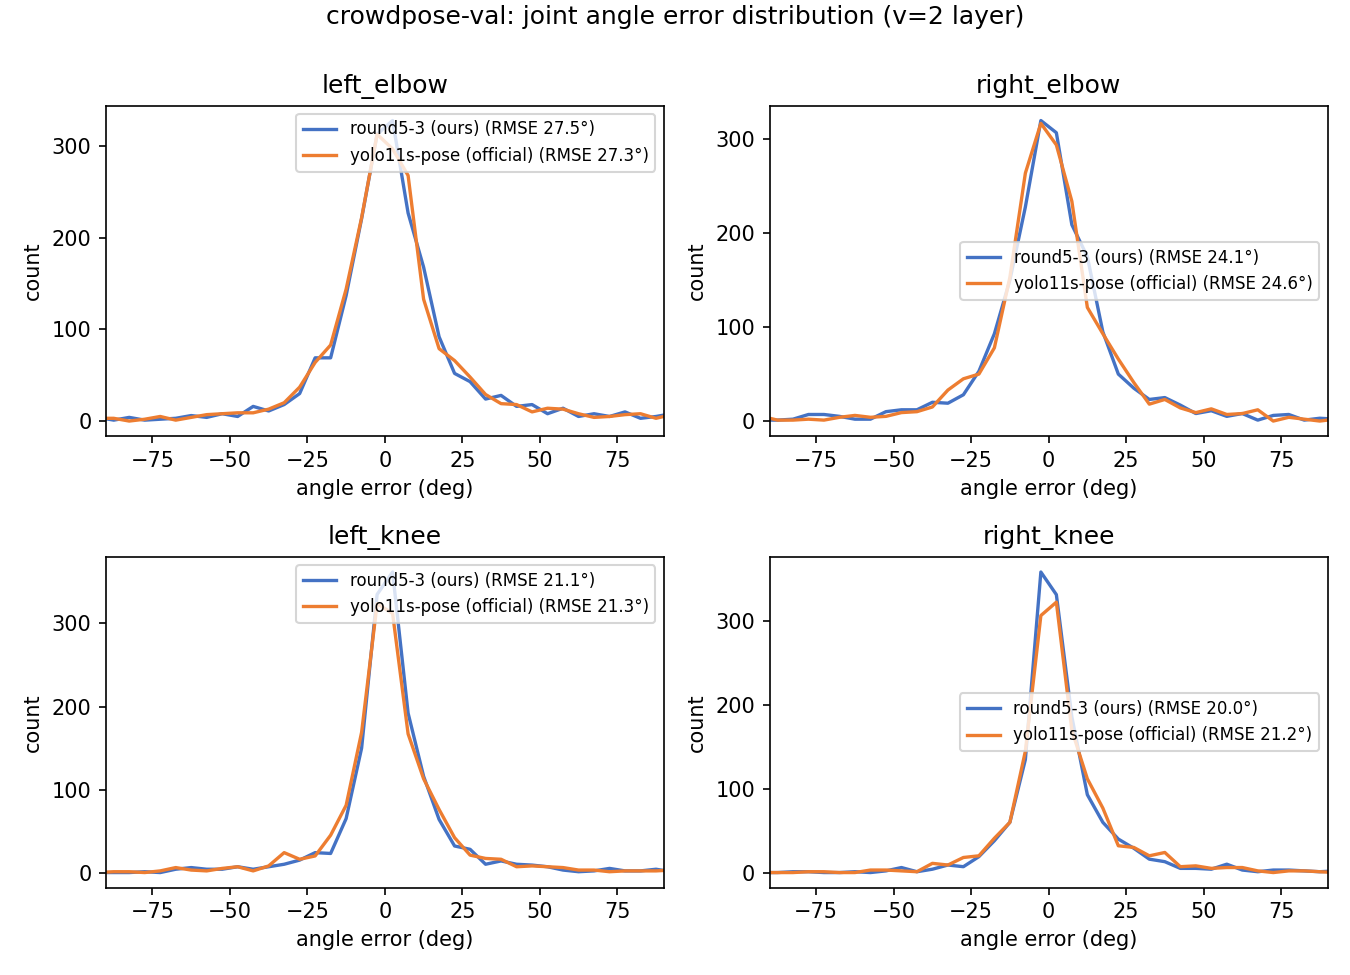
\includegraphics[width=\linewidth]{figures/fig_m2_crowdpose-val.png}
\end{minipage}\hfill
\begin{minipage}[b]{0.32\linewidth}
  \centering
  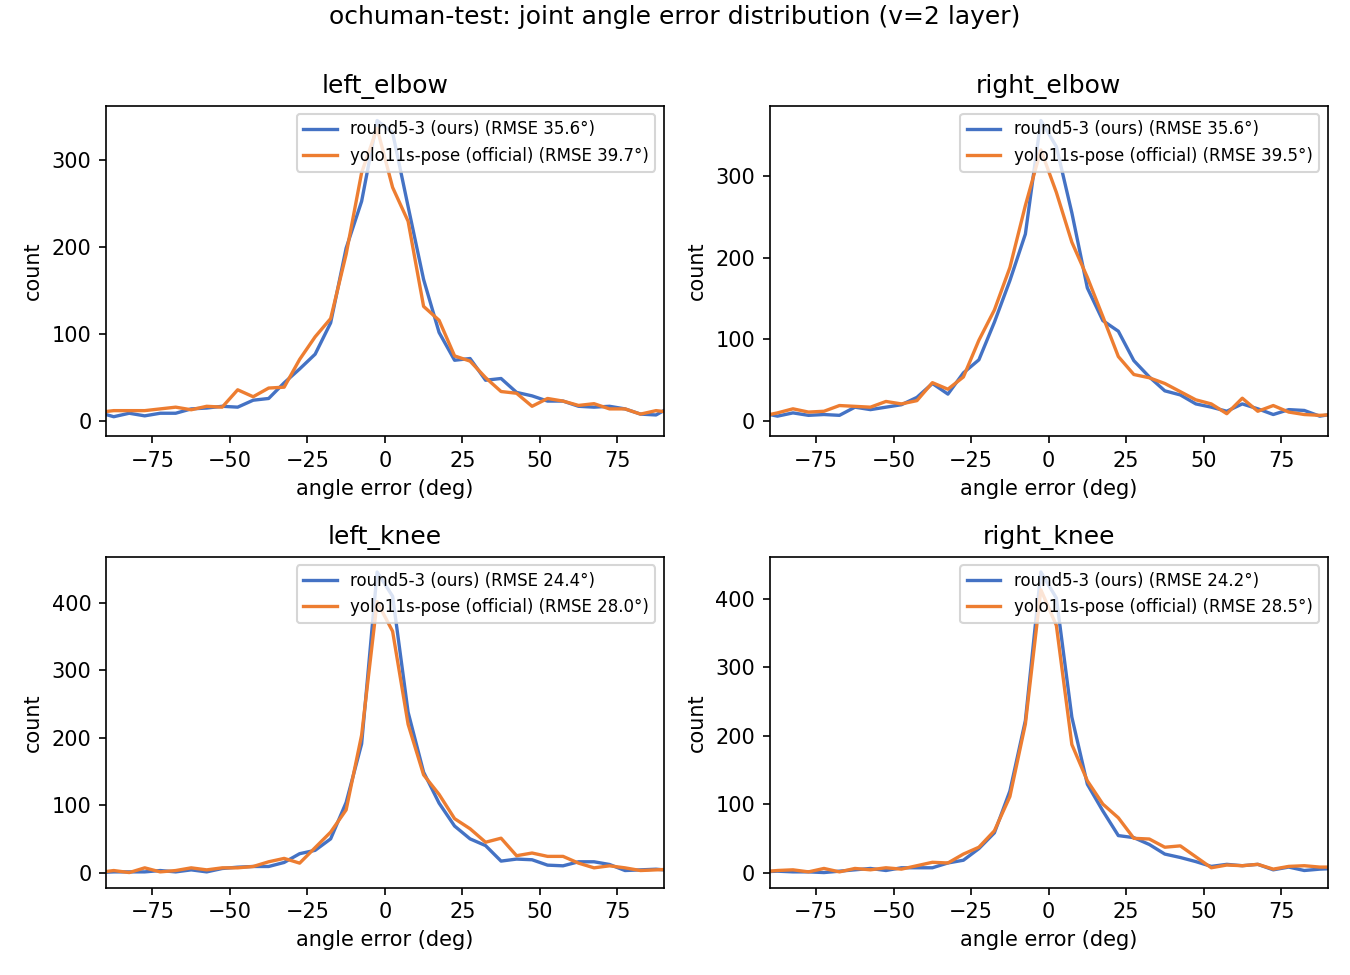
\includegraphics[width=\linewidth]{figures/fig_m2_ochuman-test.png}
\end{minipage}
\caption{M2 关节角度误差分布（$v{=}2$ 层，分数据集）：(a) COCO val2017，(b) CrowdPose val，(c) OCHuman test。每幅子图展示两模型逐关节误差直方图（$\theta_{\mathrm{pred}}-\theta_{\mathrm{gt}}$），图例含 RMSE。分布集中于 $0^{\circ}$ 附近；遮挡域数据集对两模型的区分更清晰（表~\ref{tab:m2}）。}
\label{fig:m2}
\end{figure*}

\begin{figure}[t]
\centering
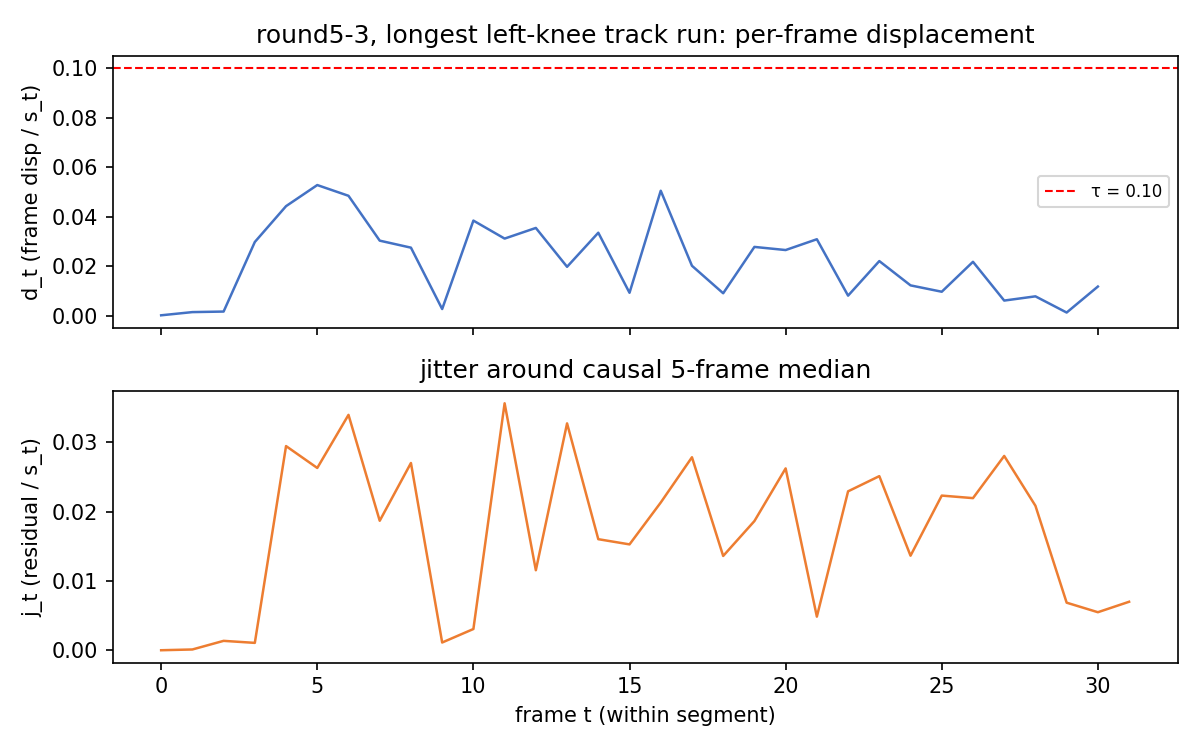
\includegraphics[width=\columnwidth]{figures/fig_m3_posetrack.png}
\caption{M3 时序抖动示例（PoseTrack18 val 一条轨迹，round5-3，最长左膝段）：（上）按人框尺度归一化的逐帧位移 $d_t$，含跳变阈值 $\tau_j=0.10$；（下）因果 5 帧中值滤波周围的残差抖动 $j_t$。}
\label{fig:m3}
\end{figure}

% =====================================================================
% 附录 A：bootstrap CI（数据来自 summary.json + extra_ci.json，中文表头）
% =====================================================================

\appendices
\renewcommand{\thetable}{A\arabic{table}}
\setcounter{table}{0}
\section{Bootstrap 置信区间}

所有区间均为 95\% 百分位 bootstrap CI，10,000 次重采样，seed 42。重采样单元：M1 与 M2 为图像（各指标在模型比较前先在该单元上聚合），M3 为轨迹段。配对比较在两量之间共享同一重采样索引；模型间比较对两模型单元独立重采样。符号约定：$\Delta=$ YOLO11s-pose $-$ round5-3，故 $\Delta<0$ 对 AP 与 $\kappa$ 表示 round5-3 占优，对 RMSE 表示 YOLO11s-pose 占优。$^{*}$ 标记不含 0 的区间。固定比较清单的每一项均列出，无挑选。

% Auto-generated by gen_appendix_tables.py. Do not edit by hand.
% 中文版：由 appendix_tables.tex 逐字翻译，数据与列结构完全一致。

\begin{table}[t]
\centering
\caption{M1 分层 AP 对比及 bootstrap 置信区间。$\Delta=$ YOLO11s-pose $-$ round5-3；$^{*}$ CI 不含 0。}
\label{tab:a1}
\renewcommand{\arraystretch}{1.15}
\resizebox{\columnwidth}{!}{%
\begin{tabular}{llccc}
\toprule
\textbf{数据集} & \textbf{层} & \textbf{AP r5-3} & \textbf{AP YOLO} & \textbf{$\Delta$ AP [95\% CI]} \\
\midrule
COCO val & full & 0.5712 & 0.5816 & 0.0104 [0.0059, 0.0155]$^{*}$ \\
COCO val & $v{=}2$ & 0.5637 & 0.5728 & 0.0091 [0.0048, 0.0144]$^{*}$ \\
COCO val & $v{=}1$ & 0.1747 & 0.1719 & -0.0028 [-0.0070, 0.0022] \\
COCO val & $v{=}0$ & 0.0000 & 0.0000 & 0.0000 [0.0000, 0.0000] \\
CrowdPose val & full & 0.7626 & 0.6938 & -0.0687 [-0.0754, -0.0616]$^{*}$ \\
CrowdPose val & $v{=}2$ & 0.4183 & 0.3768 & -0.0415 [-0.0465, -0.0362]$^{*}$ \\
CrowdPose val & $v{=}1$ & 0.5183 & 0.4573 & -0.0610 [-0.0677, -0.0540]$^{*}$ \\
CrowdPose val & $v{=}0$ & 0.0000 & 0.0000 & 0.0000 [0.0000, 0.0000] \\
OCHuman test & full & 0.4775 & 0.3379 & -0.1396 [-0.1508, -0.1281]$^{*}$ \\
OCHuman test & $v{=}2$ & 0.4696 & 0.3314 & -0.1383 [-0.1488, -0.1261]$^{*}$ \\
OCHuman test & $v{=}1$ & 0.1819 & 0.0765 & -0.1055 [-0.1153, -0.0973]$^{*}$ \\
OCHuman test & $v{=}0$ & 0.0000 & 0.0000 & 0.0000 [0.0000, 0.0000] \\
\bottomrule
\end{tabular}
}
\vspace{0.4em}\footnotesize 单位：图像（两模型共享同一图像域；配对重采样）。10,000 次重采样，seed 42，95\% 百分位 CI。
\end{table}


\begin{table}[t]
\centering
\caption{M1 $\Delta_{\mathrm{occ}}$（mAP($v{=}1$) $-$ mAP(full)）逐模型值及模型差，附 bootstrap CI。}
\label{tab:a2}
\renewcommand{\arraystretch}{1.15}
\resizebox{\columnwidth}{!}{%
\begin{tabular}{lccc}
\toprule
\textbf{数据集} & $\Delta_{\mathrm{occ}}$ r5-3 [95\% CI] & $\Delta_{\mathrm{occ}}$ YOLO [95\% CI] & $\Delta\Delta_{\mathrm{occ}}$ [95\% CI] \\
\midrule
COCO val & -0.3965 [-0.4075, -0.3858] & -0.4097 [-0.4205, -0.3989] & -0.0132 [-0.0177, -0.0086]$^{*}$ \\
CrowdPose val & -0.2443 [-0.2565, -0.2322] & -0.2366 [-0.2488, -0.2246] & 0.0077 [0.0041, 0.0110]$^{*}$ \\
OCHuman test & -0.2955 [-0.3080, -0.2842] & -0.2614 [-0.2729, -0.2527] & 0.0341 [0.0237, 0.0429]$^{*}$ \\
\bottomrule
\end{tabular}
}
\vspace{0.4em}\footnotesize 单位：图像（配对）；$\Delta\Delta_{\mathrm{occ}}$ 在配对重采样上逐元素计算。10,000 次重采样，seed 42，95\% 百分位 CI。
\end{table}


\begin{table}[t]
\centering
\caption{M2 关节角 RMSE（°，左右侧合并）及 bootstrap CI。$\Delta=$ YOLO11s-pose $-$ round5-3（负值 $=$ YOLO 误差更低）；$^{*}$ CI 不含 0。}
\label{tab:a3}
\renewcommand{\arraystretch}{1.15}
\resizebox{\columnwidth}{!}{%
\begin{tabular}{lllcccc}
\toprule
\textbf{数据集} & \textbf{关节} & \textbf{层} & \textbf{RMSE r5-3} & \textbf{RMSE YOLO} & \textbf{$\Delta$ RMSE [95\% CI]} & \textbf{$n_{\mathrm{img}}$} \\
\midrule
COCO val & 左肘 & $v{=}2$ & 27.0 & 26.3 & -0.7 [-3.1, 1.7] & 1720 / 1727 \\
COCO val & 左肘 & $v{=}1$ & 33.5 & 36.6 & 3.1 [-4.8, 10.9] & 248 / 247 \\
COCO val & 右肘 & $v{=}2$ & 24.9 & 24.5 & -0.5 [-2.8, 1.9] & 1732 / 1730 \\
COCO val & 右肘 & $v{=}1$ & 37.7 & 34.8 & -2.9 [-9.1, 3.5] & 290 / 292 \\
COCO val & 左膝 & $v{=}2$ & 20.3 & 20.9 & 0.6 [-2.0, 3.1] & 1320 / 1325 \\
COCO val & 左膝 & $v{=}1$ & 30.8 & 32.2 & 1.4 [-8.9, 11.3] & 180 / 182 \\
COCO val & 右膝 & $v{=}2$ & 20.5 & 21.2 & 0.7 [-1.6, 3.2] & 1302 / 1306 \\
COCO val & 右膝 & $v{=}1$ & 27.7 & 30.3 & 2.6 [-6.9, 12.3] & 202 / 205 \\
CrowdPose val & 左肘 & $v{=}2$ & 27.5 & 27.3 & -0.2 [-2.9, 2.6] & 790 / 793 \\
CrowdPose val & 左肘 & $v{=}1$ & 31.3 & 35.0 & 3.7 [1.4, 6.1]$^{*}$ & 1319 / 1321 \\
CrowdPose val & 右肘 & $v{=}2$ & 24.1 & 24.6 & 0.6 [-2.0, 3.2] & 810 / 811 \\
CrowdPose val & 右肘 & $v{=}1$ & 31.9 & 35.0 & 3.1 [0.7, 5.5]$^{*}$ & 1343 / 1338 \\
CrowdPose val & 左膝 & $v{=}2$ & 21.1 & 21.3 & 0.2 [-3.3, 3.7] & 575 / 575 \\
CrowdPose val & 左膝 & $v{=}1$ & 25.7 & 30.5 & 4.9 [2.1, 7.7]$^{*}$ & 1085 / 1081 \\
CrowdPose val & 右膝 & $v{=}2$ & 20.0 & 21.2 & 1.2 [-2.0, 4.4] & 570 / 571 \\
CrowdPose val & 右膝 & $v{=}1$ & 26.2 & 30.5 & 4.4 [1.4, 7.2]$^{*}$ & 1104 / 1096 \\
OCHuman test & 左肘 & $v{=}2$ & 35.6 & 39.7 & 4.2 [1.7, 6.6]$^{*}$ & 1931 / 1951 \\
OCHuman test & 左肘 & $v{=}1$ & 45.4 & 56.2 & 10.8 [7.0, 14.7]$^{*}$ & 860 / 871 \\
OCHuman test & 右肘 & $v{=}2$ & 35.6 & 39.5 & 3.9 [1.4, 6.4]$^{*}$ & 1935 / 1947 \\
OCHuman test & 右肘 & $v{=}1$ & 46.0 & 59.2 & 13.2 [9.2, 17.3]$^{*}$ & 822 / 831 \\
OCHuman test & 左膝 & $v{=}2$ & 24.4 & 28.0 & 3.6 [1.1, 6.2]$^{*}$ & 1507 / 1514 \\
OCHuman test & 左膝 & $v{=}1$ & 30.7 & 39.5 & 8.8 [3.7, 14.0]$^{*}$ & 498 / 499 \\
OCHuman test & 右膝 & $v{=}2$ & 24.2 & 28.5 & 4.3 [1.8, 6.9]$^{*}$ & 1499 / 1503 \\
OCHuman test & 右膝 & $v{=}1$ & 33.3 & 39.9 & 6.6 [0.9, 12.4]$^{*}$ & 525 / 534 \\
\bottomrule
\end{tabular}
}
\vspace{0.4em}\footnotesize 单位：图像，逐模型独立重采样（各模型的图像集只含该关节、该层至少有一个有效实例的图像）；末列 $n_{\mathrm{img}}$：round5-3 / YOLO11s-pose。10,000 次重采样，seed 42，95\% 百分位 CI。
\end{table}


\begin{table}[t]
\centering
\caption{膝内扣检出一致性（$\kappa$、灵敏度、特异度）及 bootstrap CI。$\Delta=$ YOLO11s-pose $-$ round5-3；$^{*}$ CI 不含 0。}
\label{tab:a4}
\renewcommand{\arraystretch}{1.15}
\resizebox{\columnwidth}{!}{%
\begin{tabular}{llccc cc}
\toprule
\textbf{数据集} & \textbf{$\tau_\varphi$} & \textbf{$\kappa$ r5-3 [95\% CI]} & \textbf{$\kappa$ YOLO [95\% CI]} & \multicolumn{3}{c}{\textbf{模型差 [95\% CI]}} \\
 & & & & $\Delta\kappa$ & $\Delta$ 灵敏度 & $\Delta$ 特异度 \\
\midrule
COCO val & $10^{\circ}$ & 0.724 [0.702, 0.745] & 0.697 [0.673, 0.719] & -0.027 [-0.058, 0.003] & -0.015 [-0.043, 0.014] & -0.012 [-0.029, 0.005] \\
COCO val & $15^{\circ}$ & 0.759 [0.738, 0.780] & 0.745 [0.723, 0.767] & -0.014 [-0.045, 0.016] & -0.006 [-0.039, 0.026] & -0.006 [-0.019, 0.006] \\
COCO val & $17^{\circ}$ & 0.773 [0.751, 0.794] & 0.759 [0.737, 0.780] & -0.014 [-0.045, 0.017] & -0.006 [-0.039, 0.027] & -0.006 [-0.017, 0.006] \\
CrowdPose val & $10^{\circ}$ & 0.711 [0.692, 0.729] & 0.666 [0.646, 0.685] & -0.045 [-0.073, -0.018]$^{*}$ & -0.029 [-0.052, -0.004] & -0.017 [-0.032, -0.001] \\
CrowdPose val & $15^{\circ}$ & 0.739 [0.719, 0.757] & 0.669 [0.648, 0.690] & -0.069 [-0.098, -0.041]$^{*}$ & -0.063 [-0.091, -0.034] & -0.011 [-0.024, 0.002] \\
CrowdPose val & $17^{\circ}$ & 0.731 [0.711, 0.750] & 0.665 [0.643, 0.687] & -0.067 [-0.096, -0.037]$^{*}$ & -0.067 [-0.097, -0.037] & -0.007 [-0.019, 0.005] \\
OCHuman test & $10^{\circ}$ & 0.601 [0.577, 0.625] & 0.528 [0.502, 0.554] & -0.073 [-0.108, -0.037]$^{*}$ & -0.041 [-0.072, -0.010] & -0.030 [-0.051, -0.010] \\
OCHuman test & $15^{\circ}$ & 0.602 [0.576, 0.627] & 0.519 [0.490, 0.546] & -0.084 [-0.121, -0.046]$^{*}$ & -0.054 [-0.090, -0.017] & -0.026 [-0.041, -0.011] \\
OCHuman test & $17^{\circ}$ & 0.603 [0.576, 0.628] & 0.501 [0.473, 0.530] & -0.101 [-0.140, -0.062]$^{*}$ & -0.071 [-0.110, -0.032] & -0.026 [-0.039, -0.011] \\
\bottomrule
\end{tabular}
}
\vspace{0.4em}\footnotesize 单位：图像（二值化 $\phi$ 实例按图像汇总），逐模型独立重采样。10,000 次重采样，seed 42，95\% 百分位 CI。
\end{table}


\begin{table}[t]
\centering
\caption{M3 时序指标：各域点值、模型内域差（px$-$raw、q$-$raw）及 raw 域上的模型间差，均附 bootstrap CI。$\Delta$（模型）$=$ YOLO11s-pose $-$ round5-3；$^{*}$ CI 不含 0。}
\label{tab:a5}
\renewcommand{\arraystretch}{1.15}
\resizebox{\columnwidth}{!}{%
\begin{tabular}{lccccccc}
\toprule
\textbf{指标} & \textbf{raw r5-3} & \textbf{raw YOLO} & \textbf{$\Delta$ raw} & \textbf{px$-$raw r5-3} & \textbf{px$-$raw YOLO} & \textbf{q$-$raw r5-3} & \textbf{q$-$raw YOLO} \\
\midrule
$\bar d$ & 0.0409 & 0.0430 & 0.0022 [-0.0019, 0.0062] & -0.0029 [-0.0031, -0.0027]$^{*}$ & -0.0031 [-0.0033, -0.0030]$^{*}$ & 0.0023 [0.0015, 0.0031]$^{*}$ & 0.0031 [0.0022, 0.0041]$^{*}$ \\
$\bar j$ & 0.0521 & 0.0535 & 0.0014 [-0.0047, 0.0075] & -0.0012 [-0.0013, -0.0011]$^{*}$ & -0.0013 [-0.0013, -0.0012]$^{*}$ & 0.0007 [0.0003, 0.0011]$^{*}$ & 0.0010 [0.0006, 0.0015]$^{*}$ \\
$d_{95}$ & 0.1194 & 0.1246 & 0.0051 [-0.0081, 0.0183] & -0.0086 [-0.0093, -0.0076]$^{*}$ & -0.0088 [-0.0096, -0.0080]$^{*}$ & 0.0079 [0.0050, 0.0111]$^{*}$ & 0.0103 [0.0070, 0.0140]$^{*}$ \\
$j_{95}$ & 0.1669 & 0.1719 & 0.0050 [-0.0177, 0.0275] & -0.0038 [-0.0046, -0.0032]$^{*}$ & -0.0044 [-0.0049, -0.0035]$^{*}$ & 0.0031 [0.0008, 0.0056]$^{*}$ & 0.0043 [0.0021, 0.0073]$^{*}$ \\
jump$_{0.05}$ & 0.2062 & 0.2153 & 0.0091 [-0.0145, 0.0326] & -0.0191 [-0.0206, -0.0177]$^{*}$ & -0.0210 [-0.0224, -0.0195]$^{*}$ & 0.0139 [0.0091, 0.0188]$^{*}$ & 0.0183 [0.0132, 0.0235]$^{*}$ \\
jump$_{0.10}$ & 0.0726 & 0.0777 & 0.0051 [-0.0086, 0.0190] & -0.0092 [-0.0102, -0.0082]$^{*}$ & -0.0098 [-0.0108, -0.0090]$^{*}$ & 0.0081 [0.0052, 0.0113]$^{*}$ & 0.0100 [0.0067, 0.0135]$^{*}$ \\
jump$_{0.20}$ & 0.0152 & 0.0184 & 0.0032 [-0.0015, 0.0079] & -0.0025 [-0.0030, -0.0021]$^{*}$ & -0.0030 [-0.0035, -0.0026]$^{*}$ & 0.0024 [0.0011, 0.0038]$^{*}$ & 0.0030 [0.0014, 0.0047]$^{*}$ \\
\bottomrule
\end{tabular}
}
\vspace{0.4em}\footnotesize 单位：轨迹段。域差为配对设计（跨域同一重采样索引，轨迹段由 raw 匹配固定）；模型间差对两模型轨迹段独立重采样。10,000 次重采样，seed 42（YOLO11s-pose 模型间分布为 1042），95\% 百分位 CI。
\end{table}


\begin{thebibliography}{15}
\bibitem{1} T.-Y. Lin \emph{et al.}, ``Microsoft COCO: Common objects in context,'' in \emph{Proc. ECCV}, 2014.
\bibitem{2} S.-H. Zhang \emph{et al.}, ``Pose2Seg: Detection free human instance segmentation (OCHuman),'' arXiv:1803.10683, 2018.
\bibitem{3} M. Andriluka \emph{et al.}, ``PoseTrack: A benchmark for human pose estimation and tracking,'' in \emph{Proc. CVPR}, 2018; arXiv:1712.09184, 2017.
\bibitem{4} J. Turner, J. Clark, and N. Keshtmand, ``Markerless pose estimation for resistance training technique assessment,'' arXiv:2608.24384, 2026.
\bibitem{5} Panconi \emph{et al.}, ``Deep-learning-based markerless pose estimation systems in gait analysis,'' arXiv:2407.10590, 2024.
\bibitem{6} Pemasiri \emph{et al.}, ``Biomechanically accurate gait analysis,'' arXiv:2603.02499, 2026.
\bibitem{7} J. Li \emph{et al.}, ``CrowdPose: Efficient crowded scenes pose estimation and a new benchmark,'' arXiv:1812.00324, 2018.
\bibitem{8} A. Ghafoor and A. Mahmood, ``Quantification of occlusion handling capability of a 3D human pose estimation framework,'' \emph{IEEE Trans. Multimedia}, arXiv:2203.04113, 2022.
\bibitem{9} I. S\'ar\'andi, T. Linder, K. O. Arras, and B. Leibe, ``How robust is 3D human pose estimation to occlusion?'' in \emph{Proc. IROS Workshop on Robotic Co-workers 4.0}, 2018; arXiv:1808.09316, 2018.
\bibitem{10} Y. Garg, S. Bachu, A. Dutta, R. Lal, S. Bose, C.-K. Ta, M. S. Asif, and A. Roy-Chowdhury, ``VOccl3D: A video benchmark dataset for 3D human pose and shape estimation under real occlusions,'' arXiv:2508.06757, 2025.
\bibitem{11} I. L. A. Mendon\c{c}a, F. M. do Nascimento Filho, G. Badicu, D. P. de Vasconcelos, T. B. Lima, V. Calmon, J. P. de Farias Neto, G. K. Jakubiak, L. Y. S. Maciel, F. J. Aidar, and W. Monteiro da Silva J\'unior, ``Analysis of ankle mobility and dynamic valgus knee in runners with and without patellofemoral pain syndrome,'' \emph{Health Science Reports}, vol. 9, e72051, 2026.
\bibitem{12} C. Lei \emph{et al.}, ``Deep video prior for video consistency and propagation,'' \emph{IEEE Trans. Pattern Anal. Mach. Intell.}, arXiv:2201.11632, 2022.
\bibitem{13} G. Casiez, N. Roussel, and D. Vogel, ``1\texteuro\ Filter: A simple speed-based low-pass filter for noisy input in interactive systems,'' in \emph{Proc. CHI}, 2012.
\bibitem{14} G. Jocher \emph{et al.}, ``Ultralytics YOLO11,'' \url{https://github.com/ultralytics/ultralytics}, 2024.
\bibitem{15} A. Zeng, L. Yang, X. Ju, J. Li, J. Wang, and Q. Xu, ``SmoothNet: A plug-and-play network for refining human pose estimation in videos,'' in \emph{Proc. ECCV}, 2022; arXiv:2112.13715, 2022.
\end{thebibliography}

\end{document}
